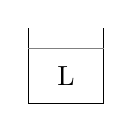
\begin{tikzpicture}[scale = 0.8]
  %%%%%%%%%%%%%The first bin%%%%%%%%%%%%%%%%%%%%%%
  \draw (0,1.2) -- (0,0) -- (1.2,0)--(1.2,1.2);
  \draw[gray] (0,0.88) -- (1.2,0.88);
  \draw node at (0.6,0.44) {L};
\end{tikzpicture}
\quad
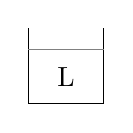
\begin{tikzpicture}[scale = 0.8]
  %%%%%%%%%%%%%The second bin%%%%%%%%%%%%%%%%%%%%%%
  \draw (0,1.2) -- (0,0) -- (1.2,0)--(1.2,1.2);
  \draw[gray] (0,0.86) -- (1.2,0.86);
  \draw node at (0.6,0.43) {L};
\end{tikzpicture}
\quad
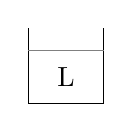
\begin{tikzpicture}[scale = 0.8]
  %%%%%%%%%%%%%The third bin%%%%%%%%%%%%%%%%%%%%%%
  \draw (0,1.2) -- (0,0) -- (1.2,0)--(1.2,1.2);
  \draw[gray] (0,0.84) -- (1.2,0.84);
  \draw node at (0.6,0.42) {L};
\end{tikzpicture}
\quad
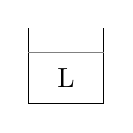
\begin{tikzpicture}[scale = 0.8]
  %%%%%%%%%%%%%The forth bin%%%%%%%%%%%%%%%%%%%%%%
  \draw (0,1.2) -- (0,0) -- (1.2,0)--(1.2,1.2);
  \draw[gray] (0,0.82) -- (1.2,0.82);
  \draw node at (0.6,0.41) {L};
\end{tikzpicture}
  
  